\begin{center}
	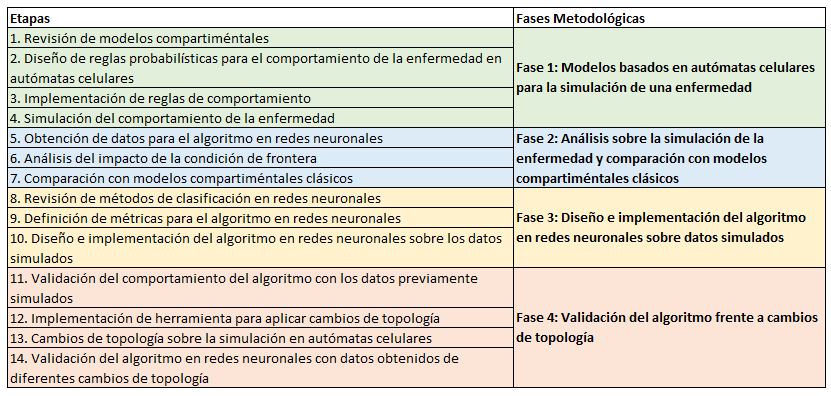
\includegraphics[width=1\linewidth]{Imagenes/fasesMetodologicas.PNG}
\end{center}

\subsubsection*{Fase 1: Modelos basados en autómatas celulares para la simulación de una enfermedad.}
La primera fase del proyecto consistirá en simular el comportamiento de la enfermedad sobre un autómata celular. Para alcanzar este objetivo, será necesario comprender las dinámicas que describen los modelos SIS, SIR y algunas de sus variaciones. Esto permitirá definir las reglas probabilísticas que en conjunto, describirán la propagación de la enfermedad de modo que se tengan en cuenta las interacciones de cada célula.

Inicialmente se trabajará sobre una red uniforme, en donde se consideren las vecindades de Moore o las de Von Neumann.

\subsubsection*{Fase 2: Análisis sobre la simulación de la enfermedad y comparación con modelos compartiméntales clásicos.}
Una vez se llegue a un entorno de simulación estable, se realizarán modificaciones en la condición de frontera para posteriormente analizar su impacto en la propagación de la enfermedad.

A continuación se realizarán comparaciones entre la simulación y los modelos compartiméntales clásicos. Esto permitirá validar el comportamiento simulado, de acuerdo con la manera en la que se diseñen las reglas de comportamiento en la fase 1.

\subsubsection*{Fase 3: Diseño e implementación del algoritmo en redes neuronales sobre datos simulados.}
Durante esta fase del proyecto, se realizará inicialmente un ejercicio investigativo en modelos de clasificación. Esto permitirá comprender la manera en la que se definen las métricas, que posteriormente serán monitoreadas por el algoritmo en redes neuronales.
Tan pronto como se definan las métricas, se dará inicio en paralelo, al diseño e implementación del algoritmo en redes neuronales.

\subsubsection*{Fase 4: Validación del algoritmo frente a cambios de topología.}
Daremos inicio a la fase final del proyecto, con la validación del algoritmo desarrollado en la fase anterior. Las pruebas realizadas durante esta validación, se elaborarán sobre los datos obtenidos de las simulaciones realizadas en la primera fase.